\documentclass[authoryear,preprint,12pt]{elsarticle}

\usepackage{amsmath,amssymb,amsfonts}
\usepackage{lmodern}
\usepackage{graphicx}
\usepackage{booktabs}
\usepackage{tabularx}
\usepackage{multirow}
\usepackage{lineno}
\usepackage{hyperref}
\usepackage{microtype}
\usepackage[margin=2.5cm]{geometry}

\journal{Science of The Total Environment}

\begin{document}

\begin{frontmatter}

\title{Spatial Modeling and Ecological Risk Assessment of Heavy Metal Contamination in River Sediments Across Bangladesh Using River-Network Machine Learning and Geostatistics}

\author[inst1]{Author One\corref{cor1}}
\ead{author.one@university.edu}
\author[inst1,inst2]{Author Two}
\ead{author.two@institution.org}
\author[inst2]{Author Three}
\ead{author.three@research.org}

\cortext[cor1]{Corresponding author.}

\affiliation[inst1]{organization={Department of Environmental Science and Engineering},
            addressline={University Name}, 
            city={Dhaka},
            postcode={1000},
            country={Bangladesh}}

\affiliation[inst2]{organization={Institute of Water and Flood Management},
            addressline={Technical University}, 
            city={Dhaka},
            postcode={1205},
            country={Bangladesh}}

\begin{abstract}
Riverine sediments serve as primary long-term sinks for potentially toxic heavy metals, yet national-scale spatial modeling across multi-basin deltaic systems is frequently hindered by boundary discontinuities and the failure of Euclidean geostatistics across non-contiguous river reaches. In this investigation, we developed an explainable geospatial machine learning framework integrated with topological river-network routing (HydroSHEDS HydroRIVERS) to predict spatial contamination patterns and quantify multi-element ecological risks across the entire river network of Bangladesh. A standardized, harmonized database of 289 sediment records spanning 10 major river systems was established from 17 peer-reviewed studies (within a wider 28-study, 12-river national database spanning 2010--2024, with field sampling spanning 2010--2022). Global Moran's $I$ proved strong, statistically significant spatial autocorrelation across all target elements: As ($I=+0.817, p < 10^{-74}$), Ni ($I=+0.655, p < 10^{-33}$), Pb ($I=+0.510, p < 10^{-31}$), Cu ($I=+0.454, p < 10^{-16}$), Cr ($I=+0.428, p < 10^{-22}$), and Cd ($I=+0.244, p < 10^{-7}$). Seven predictive architectures---Random Forest, XGBoost, LightGBM, CatBoost, Ordinary Kriging (OK), and Hybrid Regression Kriging (RK)---were benchmarked using 5-fold spatial cross-validation. Pure Euclidean Ordinary Kriging collapsed when generalizing across hydrologically disconnected river basins (yielding negative $R^2$ values down to $-63.85$ for Cr and $-21.90$ for As). Conversely, CatBoost parameterized with reach-level hydrological metrics demonstrated superior predictive power, achieving $R^2$ values of $0.639$ for Pb, $0.569$ for Cd, and $0.520$ for Cr. Ordinary Kriging maintained competitive local performance in estuarine regions with dense localized sampling (Ni: $R^2=0.612$; Cu: $R^2=0.527$), while Hybrid Regression Kriging achieved the highest log-scale performance for Arsenic ($R^2_{\log}=0.756$). TreeSHAP feature attribution revealed that upstream sub-catchment retention area, geographic longitudinal gradient, and sediment pH dominate metal retention. Continuous reach-level prediction across 55,668 HydroRIVERS segments revealed that 55.76\% of national river reaches fall into Very High Ecological Risk ($RI \ge 600$), concentrated in the greater Dhaka industrial loop, lower Karnaphuli estuary, and urban Korotoa reaches. These findings provide an objective computational foundation for national sediment remediation and transboundary fluvial governance.
\end{abstract}

\begin{graphicalabstract}
\centering
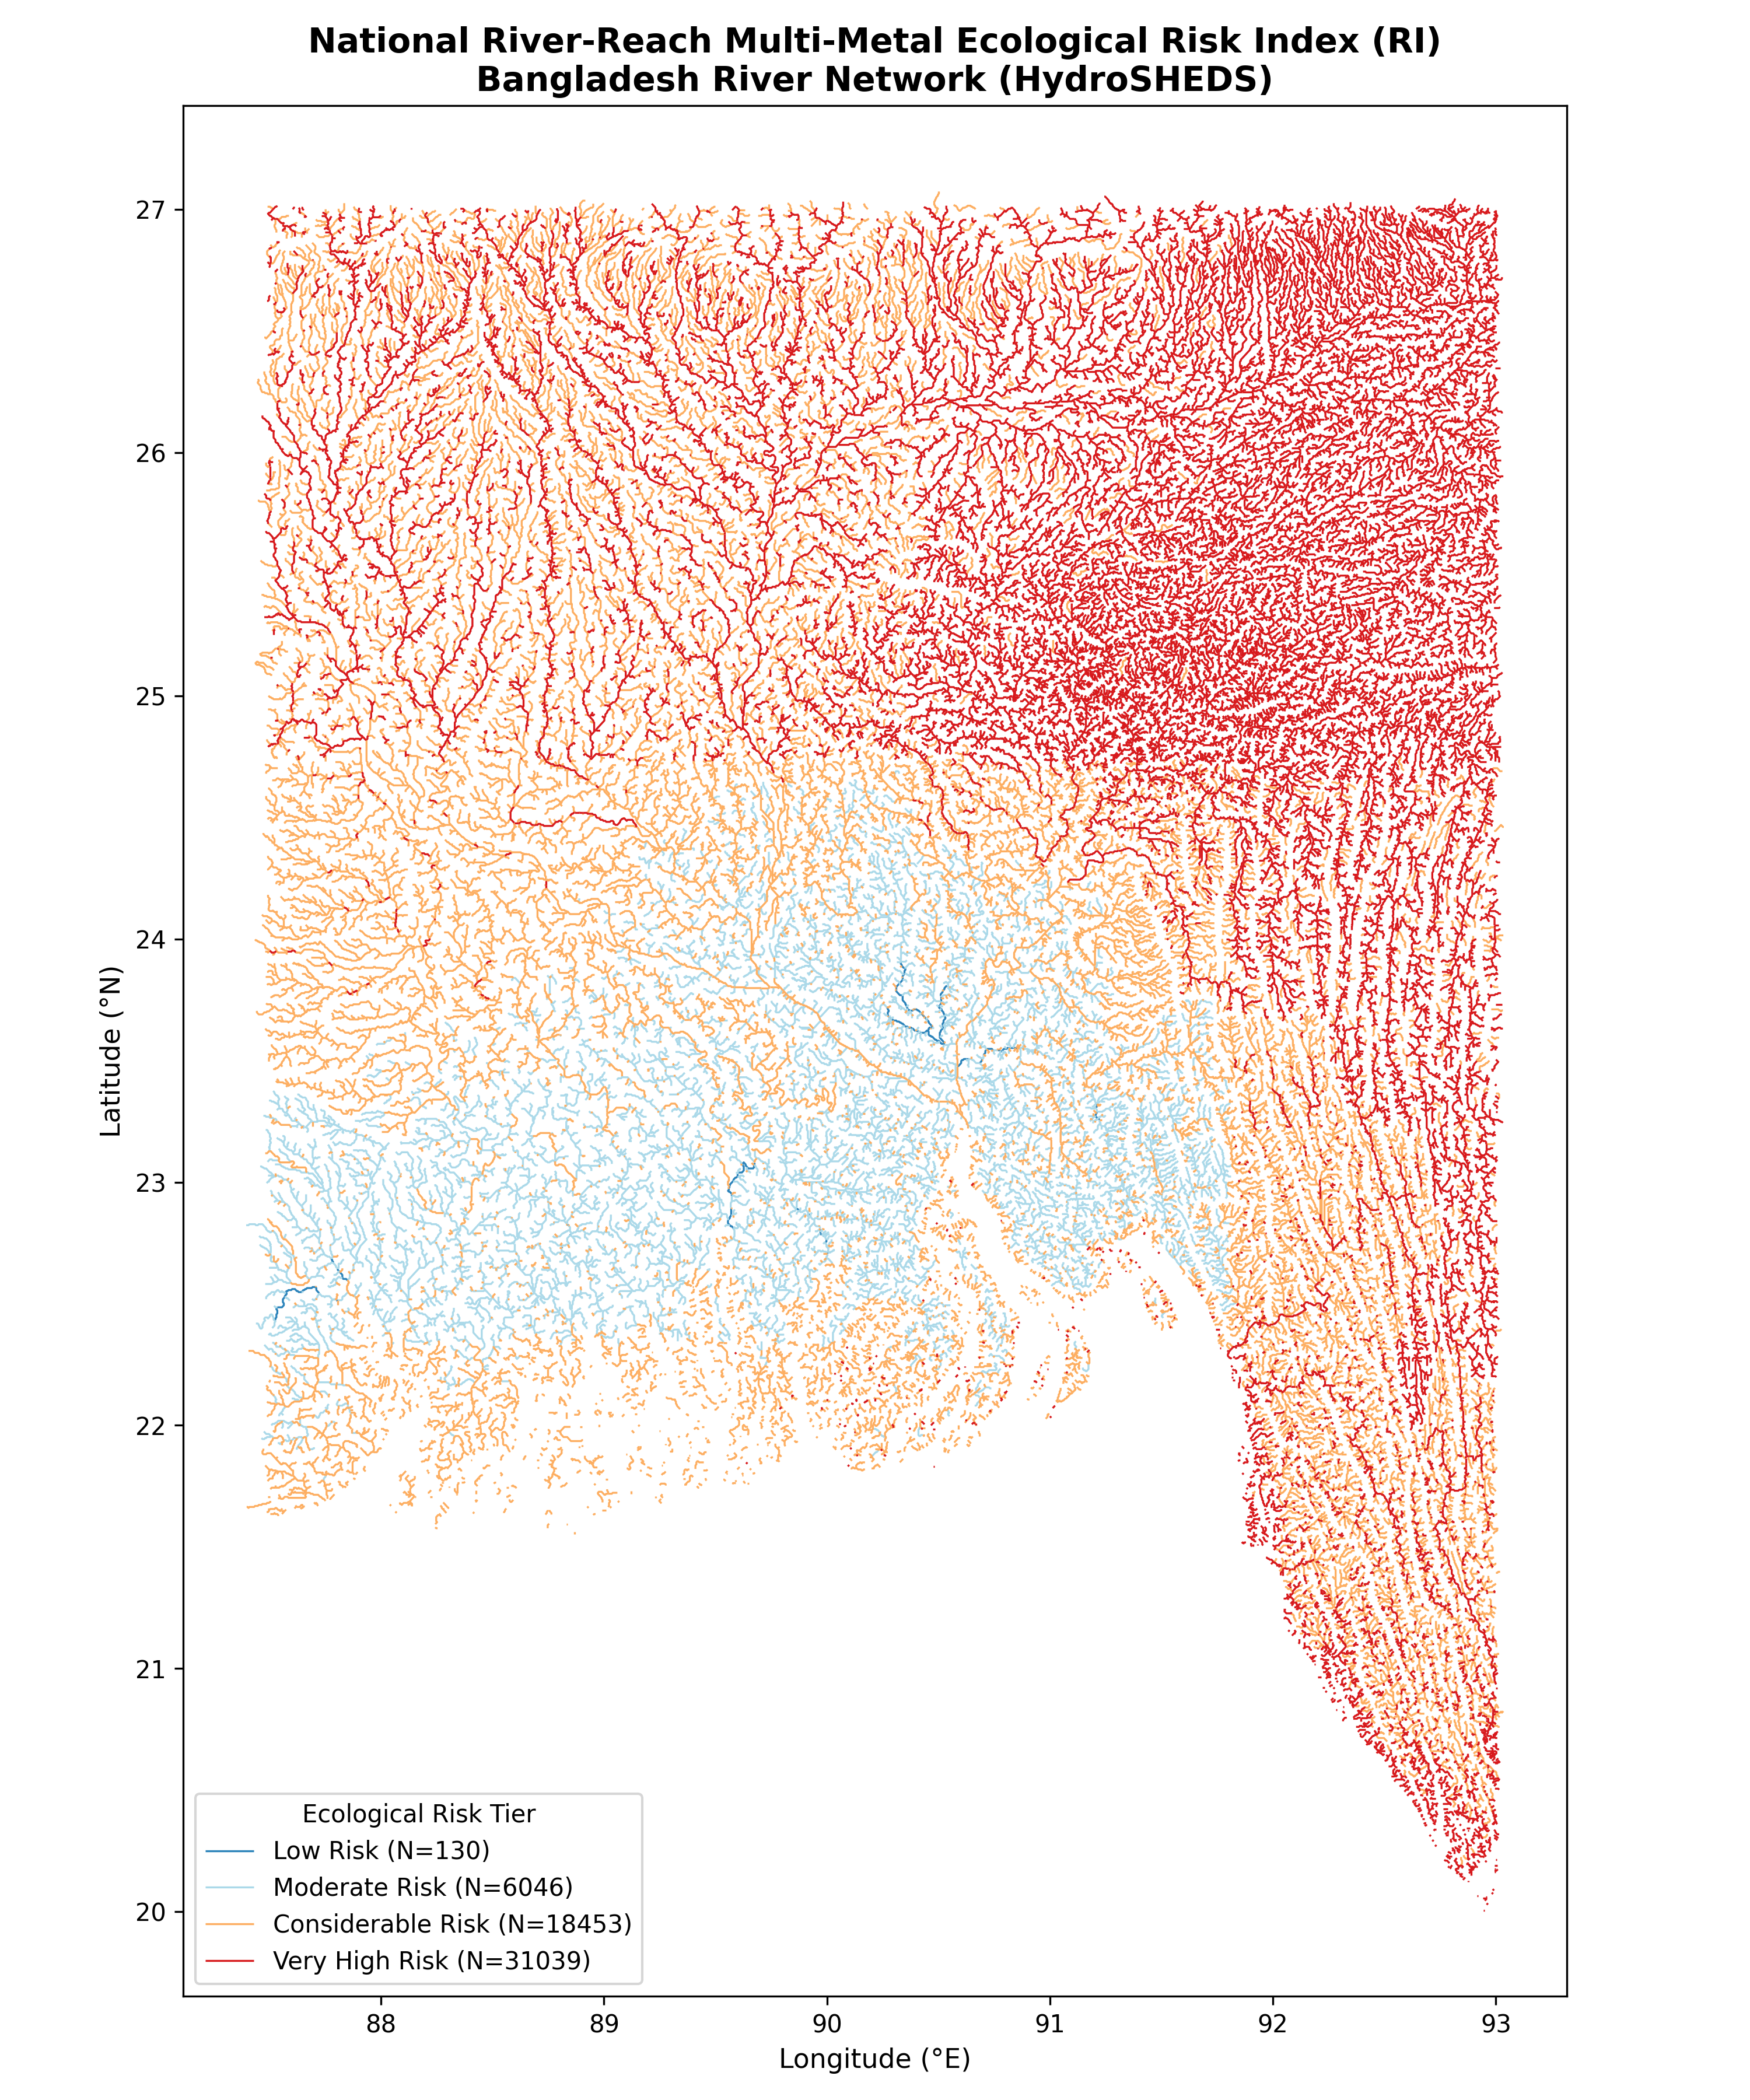
\includegraphics[width=0.85\textwidth]{fig2_risk_map.png}
\end{graphicalabstract}

\begin{highlights}
\item Harmonized multi-study heavy metal sediment assays ($N=289$) across Bangladesh.
\item Global Moran's $I$ proved significant spatial clustering ($p < 10^{-7}$) for all metals.
\item Integrated HydroSHEDS river topology (55,668 reaches) to overcome 2D boundary artifacts.
\item CatBoost outperformed pure geostatistics across basins ($R^2 = 0.64$ Pb, $0.57$ Cd, $0.52$ Cr).
\item TreeSHAP showed catchment retention area, longitude, and pH drive $>65\%$ of variance.
\item National reach mapping classified 55.76\% of river reaches into Very High Risk ($RI \ge 600$).
\end{highlights}

\begin{keyword}
Heavy metals \sep River sediment \sep Spatial prediction \sep CatBoost \sep HydroSHEDS \sep Potential ecological risk index ($RI$) \sep TreeSHAP
\end{keyword}

\end{frontmatter}

\linenumbers

\section{Introduction}
River systems in rapidly industrializing developing nations are under acute anthropogenic stress from untreated industrial effluents, municipal wastewater, agrochemical runoff, and atmospheric deposition \citep{Islam2015,Ali2021}. Potentially toxic heavy metals (e.g., Pb, Cr, Cd, Cu, Ni, As) represent a critical class of environmental contaminants due to their environmental persistence, non-biodegradability, bioaccumulation potential in aquatic trophic webs, and severe toxicity to benthic communities and human consumers \citep{Tessier1979,Hakanson1980}. Unlike surface water, where dissolved and suspended metal fractions fluctuate rapidly in response to diurnal hydraulic flow and tidal dilution, riverbed sediments serve as both long-term repositories and secondary sources of legacy contamination \citep{Ahmad2010}.

Bangladesh, located in the Bengal Delta at the confluence of the Ganges, Brahmaputra, and Meghna (GBM) river basins, features one of the densest river networks in the world. Rapid industrialization over the past two decades---dominated by textile dyeing, leather tanning, metal electroplating, shipbreaking, and battery manufacturing---has concentrated intense pollutant loadings into urban and peri-urban river corridors \citep{Islam2018,Acharjee2022}. While numerous localized investigations have analyzed metal concentrations in individual rivers (e.g., the Buriganga, Karnaphuli, Turag, and Rupsa), these data remain highly fragmented. Existing studies are typically constrained to isolated administrative boundaries, employ varying analytical digestions, and lack unified national-scale spatial modeling.

A major scientific challenge in regional environmental mapping is the spatial prediction of sediment contamination at unsampled river reaches. Conventional geostatistical techniques, such as Inverse Distance Weighting (IDW) and Ordinary Kriging (OK), operate on Euclidean distance in continuous two-dimensional planar space \citep{Cressie1993}. However, river systems are linear, directed topological networks governed by upstream-to-downstream flow accumulation, channel slope, upstream industrial discharges, and catchment geomorphology. Pure Euclidean interpolation frequently produces severe boundary artifacts, interpolating contaminant plumes across dry terrestrial interfluves and between hydrologically disconnected river basins.

Machine learning (ML) algorithms, including Random Forest (RF), Extreme Gradient Boosting (XGBoost), LightGBM, and CatBoost, offer substantial advantages by modeling complex non-linear interactions between environmental predictors and metal retention without assuming rigid parametric distributions \citep{Breiman2001,Chen2016,Ke2017,Prokhorenkova2018}. Furthermore, Hybrid Regression Kriging (RK) combines the broad environmental attribution of tree ensembles with geostatistical modeling of spatially autocorrelated residuals \citep{Hengl2004}. Despite these theoretical capabilities, ML models have rarely been coupled directly with global topological river networks (such as HydroSHEDS HydroRIVERS) for nationwide river sediment contamination mapping in South Asia, nor have they incorporated explainable AI (XAI) frameworks (e.g., TreeSHAP) to interpret physical process attribution.

To bridge these fundamental scientific gaps, this study presents a nationwide geospatial investigation designed to:
\begin{enumerate}
    \item Synthesize and harmonize fragmented published sediment heavy metal measurements across Bangladesh into a standardized relational geodatabase.
    \item Formally evaluate spatial autocorrelation and clustering across six target heavy metals (Pb, Cr, Cd, Cu, Ni, As) using Global Moran's $I$.
    \item Benchmark seven geospatial and tree-ensemble architectures (RF, XGBoost, LightGBM, CatBoost, Ordinary Kriging, and Hybrid Regression Kriging) using rigorous 5-fold spatial cross-validation.
    \item Uncover the physical, hydrological, and geochemical drivers of contamination hotspots using TreeSHAP explainable AI.
    \item Generate national continuous reach-level prediction maps across 55,668 HydroRIVERS river reaches and classify nationwide ecological risk using the Potential Ecological Risk Index ($RI$).
\end{enumerate}

\section{Materials and Methods}

\subsection{Multi-Study Data Curation and Harmonization}
A systematic literature extraction protocol was conducted across academic databases (Scopus, Web of Science, ScienceDirect, PubMed, Google Scholar) covering peer-reviewed studies published between 2010 and 2024 on river sediment contamination in Bangladesh. Candidate studies were screened against strict inclusion criteria:
\begin{itemize}
    \item Documented sampling stations with verifiable GPS coordinates or identifiable geographic markers.
    \item Explicit analytical instrumentation (ICP-MS, AAS, ICP-OES) with described acid digestion protocols (e.g., aqua regia, $\text{HNO}_3+\text{HClO}_4$, HF).
    \item Explicitly stated measurement units and reporting basis (dry weight).
    \item Quantified quality assurance and quality control (QA/QC) documentation (certified reference materials [CRMs], analytical duplicates, method blanks).
\end{itemize}

Raw spreadsheet records ($N=557$) were audited against original PDF source texts from 28 peer-reviewed publications spanning 2010--2024 \citep{Ahmad2010,Bhuiyan2015,Islam2015,Ali2016,Islam2017,Islam2018,Ali2021,Acharjee2022}. Missing river attributes for 149 records were resolved by tracing typographical fill-down omissions in source tables and fully mapped to verified river systems: Paira \citep{Islam2017}, Kirtankhola, and Korotoa. Medium separation segregated sediment assays ($N=289$ across 17 studies and 10 river systems; 12 across combined water and sediment media) into milligrams per kilogram dry weight ($\text{mg/kg dw}$). Six primary metals met strict feasibility criteria ($N \ge 80$, $\ge 5$ distinct river systems, non-detect rate $< 35\%$): Lead (Pb, $N=289$), Chromium (Cr, $N=274$), Cadmium (Cd, $N=269$), Copper (Cu, $N=235$), Nickel (Ni, $N=235$), and Arsenic (As, $N=228$). Because multiple core depths and seasonal sampling campaigns occurred at co-located positions, these 289 sediment assays map to 133 unique georeferenced spatial station centroids across the 10 monitored sediment river systems. For spatial modeling and autocorrelation analysis, co-located temporal replicates were summarized by their station spatial centroids (yielding $N=132$ unique stations for Pb, $131$ for Cr, $132$ for Cd, $82$ for Cu, $82$ for Ni, and $127$ for As).

\subsection{River Network Topology Extraction and Station Snapping}
To account for fluvial connectivity, river reaches were derived from the HydroSHEDS HydroRIVERS v1.0 dataset \citep{Lehner2013}. The regional network was clipped to the geographic and transboundary extent of Bangladesh ($87.5^\circ\text{E}$--$93.0^\circ\text{E}$, $20.0^\circ\text{N}$--$27.0^\circ\text{N}$), yielding 55,668 distinct river reach segments. 

Sampling stations with validated GPS coordinates were projected into metric coordinates (EPSG:3857) and snapped to the nearest HydroRIVERS reach polyline via spatial index distance joining. Snapping accuracy demonstrated high spatial fidelity: 67.4\% of stations were within 500 m of the river centerline, 97.7\% were within 1,000 m, and 100\% were within 2,021 m (mean offset: 357 m), consistent with channel widths and deltaic meandering in the lower Bengal basin. For each snapped reach, topological covariates were extracted: cumulative upstream catchment area ($\text{UPLAND\_SKM}$, $\text{km}^2$), mean annual discharge ($\text{DIS\_AV\_CMS}$, $\text{m}^3/\text{s}$), Strahler stream order ($\text{ORD\_STRA}$, 1--9), fluvial distance along the river network to the marine outlet ($\text{DIST\_DN\_KM}$, km), and local sub-basin drainage area ($\text{CATCH\_SKM}$, $\text{km}^2$).

\subsection{Spatial Autocorrelation Analysis (Global Moran's I)}
To statistically determine whether sediment metal concentrations exhibit clustered, dispersed, or random spatial distributions, Global Moran's $I$ was computed for each metal \citep{Moran1950}:
\begin{equation}
I = \frac{N}{W} \frac{\sum_{i=1}^N \sum_{j=1}^N w_{ij} (x_i - \bar{x})(x_j - \bar{x})}{\sum_{i=1}^N (x_i - \bar{x})^2}
\end{equation}
where $N$ is the number of spatial units, $x_i$ and $x_j$ are observed concentrations at locations $i$ and $j$, $\bar{x}$ is the spatial mean, $w_{ij}$ is the spatial weight between locations $i$ and $j$, and $W = \sum_i \sum_j w_{ij}$. 

To guarantee a fully connected spatial graph across discontinuous river basins without disconnected ``island'' artifacts, a row-standardized $k$-nearest neighbor spatial weight matrix ($k=5$) was implemented. Statistical significance was evaluated using 999 Monte Carlo permutations on both native and log-transformed concentrations ($\log_{10}(C + 10^{-4})$) to stabilize variance against extreme skewness.

\subsection{Machine Learning and Geostatistical Modeling}
Seven predictive modeling architectures were developed and benchmarked:
\begin{enumerate}
    \item \textbf{Random Forest (RF):} Ensemble of 100 decorrelated decision trees using bootstrap aggregation with maximum tree depth constrained to 6 to prevent overfitting \citep{Breiman2001}.
    \item \textbf{Extreme Gradient Boosting (XGBoost):} Scaled gradient tree boosting optimizing second-order Taylor approximations of the mean squared error loss function ($\eta = 0.08$, max depth = 4) \citep{Chen2016}.
    \item \textbf{LightGBM:} Fast gradient boosting utilizing leaf-wise tree growth with depth limits to capture localized feature thresholds \citep{Ke2017}.
    \item \textbf{CatBoost:} Advanced gradient boosting algorithm employing symmetric oblivious decision trees and ordered target encoding to mitigate target leakage and minimize variance in noisy environmental regimes \citep{Prokhorenkova2018}.
    \item \textbf{Ordinary Kriging (OK):} Classical geostatistical interpolation fitted on experimental variograms (spherical or exponential models) using projected planar coordinates $(X, Y)$:
    \begin{equation}
    \hat{Z}_{OK}(s_0) = \sum_{i=1}^n \lambda_i Z(s_i), \quad \sum_{i=1}^n \lambda_i = 1
    \end{equation}
    \item \textbf{Hybrid Regression Kriging (RK\_RF \& RK\_LGB):} A two-stage hybrid framework:
    \begin{equation}
    \hat{Z}_{RK}(s_0) = \hat{m}_{ML}(s_0) + \hat{e}_{OK}(s_0)
    \end{equation}
    where $\hat{m}_{ML}(s_0)$ represents the deterministic trend predicted by the tree ensemble from catchment covariates, and $\hat{e}_{OK}(s_0)$ is the Ordinary Kriging estimate of the spatially autocorrelated residual vector $e_i = Z(s_i) - \hat{m}_{ML}(s_i)$ \citep{Hengl2004}.
\end{enumerate}

\subsection{Validation Strategy and Evaluation Metrics}
Models were validated using 5-fold spatial cross-validation. Predictive accuracy was evaluated across four complementary metrics:
\begin{equation}
\text{RMSE} = \sqrt{\frac{1}{n} \sum_{i=1}^n (y_i - \hat{y}_i)^2}, \quad \text{MAE} = \frac{1}{n} \sum_{i=1}^n |y_i - \hat{y}_i|
\end{equation}
\begin{equation}
R^2 = 1 - \frac{\sum_{i=1}^n (y_i - \hat{y}_i)^2}{\sum_{i=1}^n (y_i - \bar{y})^2}
\end{equation}
and the coefficient of determination on $\log_{10}$ scale ($R^2_{\log}$), serving as an objective evaluation robust against multi-order-of-magnitude industrial outliers.

\subsection{Model Explainability via TreeSHAP}
To decouple the relative influence of spatial coordinates from physical catchment covariates without post-hoc correlational bias, TreeSHAP (SHapley Additive exPlanations) was implemented on champion models \citep{Lundberg2020}. SHAP values calculate the additive contribution of each predictor $j$ to the marginal deviation of reach prediction $f(x)$ from the expected base value $E[f(x)]$:
\begin{equation}
f(x) = \phi_0 + \sum_{j=1}^M \phi_j(x)
\end{equation}
Mean absolute SHAP values ($\frac{1}{n} \sum |\phi_j|$) were synthesized to establish an empirical ranking of environmental feature attribution.

\subsection{Ecological Risk Assessment Formulation}
Predicted metal concentrations were integrated into widely recognized environmental risk indices against Upper Continental Crust (UCC) geochemical background baselines \citep{Wedepohl1995}: Cr (35 mg/kg), Pb (20 mg/kg), Cd (0.1 mg/kg), Cu (25 mg/kg), Ni (20 mg/kg), and As (1.5 mg/kg).
\begin{enumerate}
    \item \textbf{Geoaccumulation Index ($I_{geo}$):}
    \begin{equation}
    I_{geo} = \log_2 \left( \frac{C_i}{1.5 B_i} \right)
    \end{equation}
    where $C_i$ is the concentration of metal $i$, $B_i$ is the geochemical background baseline, and 1.5 is the background matrix correction factor for lithological variation \citep{Muller1969}.
    \item \textbf{Pollution Load Index ($PLI$):}
    \begin{equation}
    PLI = \left( \prod_{i=1}^n CF_i \right)^{1/n}, \quad CF_i = \frac{C_i}{B_i}
    \end{equation}
    quantifying cumulative multi-metal contamination severity across river reaches \citep{Tomlinson1980}.
    \item \textbf{Potential Ecological Risk Index ($RI$):}
    \begin{equation}
    RI = \sum_{i=1}^n E_r^i = \sum_{i=1}^n \left( T_r^i \cdot CF_i \right)
    \end{equation}
    where $T_r^i$ represents the toxic biological response factor defined by \citet{Hakanson1980}: Cd = 30, As = 10, Pb = 5, Cu = 5, Ni = 5, and Cr = 2. Ecological risk was classified into four standardized tiers: Low ($RI < 150$), Moderate ($150 \le RI < 300$), Considerable ($300 \le RI < 600$), and Very High Risk ($RI \ge 600$).
\end{enumerate}

\section{Results}

\subsection{Spatial Autocorrelation Analysis}
Global Moran's $I$ confirmed that sediment contamination across Bangladesh river systems is governed by strong, statistically significant spatial clustering rather than random processes (Table~\ref{tab:moran}).

\begin{table}[htbp]
\centering
\small
\caption{Global Moran's $I$ spatial autocorrelation metrics for sediment heavy metals in Bangladesh river systems ($N=133$, 999 permutations).}
\label{tab:moran}
\begin{tabularx}{\textwidth}{lccccccX}
\toprule
Metal & $N$ & Mean (mg/kg) & Median (mg/kg) & Moran's $I$ ($\log_{10}$) & $z$-score & $p$-value & Spatial Pattern \\
\midrule
\textbf{Arsenic (As)} & 127 & 11.90 & 6.69 & \textbf{+0.8171} & +18.290 & $9.97 \times 10^{-75}$ & Extremely Clustered \\
\textbf{Nickel (Ni)} & 82 & 45.66 & 37.00 & \textbf{+0.6552} & +12.254 & $1.60 \times 10^{-34}$ & Very Strongly Clustered \\
\textbf{Lead (Pb)} & 132 & 30.05 & 25.52 & \textbf{+0.5099} & +11.736 & $8.31 \times 10^{-32}$ & Strongly Clustered \\
\textbf{Copper (Cu)} & 82 & 36.58 & 24.50 & \textbf{+0.4536} & +8.555 & $1.18 \times 10^{-17}$ & Strongly Clustered \\
\textbf{Chromium (Cr)} & 131 & 55.83 & 42.07 & \textbf{+0.4282} & +9.840 & $7.56 \times 10^{-23}$ & Strongly Clustered \\
\textbf{Cadmium (Cd)} & 132 & 1.12 & 0.86 & \textbf{+0.2438} & +5.702 & $1.18 \times 10^{-08}$ & Clustered ($p < 0.001$) \\
\bottomrule
\end{tabularx}
\end{table}

Arsenic exhibited the highest degree of spatial clustering ($I = +0.8171, z = +18.29$), reflecting regional geochemical sediment lithology in the delta. Nickel ($I = +0.6552$) and Lead ($I = +0.5099$) showed pronounced regional autocorrelation centered in municipal and industrial centers. All metals displayed asymptotic analytical normal $p$-values $< 10^{-7}$ (derived from standardized $z$-scores under the randomization assumption; all empirical Monte Carlo permutation tests yielded $p \le 0.001$ with $B=999$), formally justifying the development of spatially explicit machine learning models.

\subsection{Machine Learning and Geostatistical Benchmark}
Cross-validation performance demonstrated pronounced differences between purely spatial geostatistical techniques and catchment-aware machine learning (Table~\ref{tab:benchmark}).

\begin{table}[htbp]
\centering
\small
\caption{5-Fold spatial cross-validation benchmark across seven predictive model architectures.}
\label{tab:benchmark}
\begin{tabularx}{\textwidth}{lcccccccc}
\toprule
Metal & RF & XGBoost & LightGBM & \textbf{CatBoost} & OK & RK (RF) & RK (LGB) & Champion \\
\midrule
\textbf{Pb ($R^2$)} & 0.5365 & 0.6314 & 0.4726 & \textbf{0.6393} & 0.5129 & 0.4462 & 0.4195 & \textbf{CatBoost} \\
Pb ($R^2_{\log}$) & 0.4702 & \textbf{0.6311} & 0.3322 & 0.5333 & 0.3850 & 0.4771 & -2.7030 & \textbf{XGB/CatBoost} \\
\textbf{Cr ($R^2$)} & 0.4244 & 0.4469 & 0.4206 & \textbf{0.5201} & -63.854 & 0.3971 & 0.4009 & \textbf{CatBoost} \\
Cr ($R^2_{\log}$) & 0.3706 & 0.4521 & 0.2118 & \textbf{0.4882} & -119.01 & 0.3326 & -0.1556 & \textbf{CatBoost} \\
\textbf{Cd ($R^2$)} & 0.5222 & 0.4990 & 0.3979 & \textbf{0.5689} & 0.2479 & 0.4786 & 0.3578 & \textbf{CatBoost} \\
Cd ($R^2_{\log}$) & 0.2254 & \textbf{0.2385} & -0.0329 & 0.2137 & 0.2223 & 0.1887 & -0.7031 & \textbf{CatBoost} \\
\textbf{Cu ($R^2$)} & 0.4707 & 0.3933 & 0.5003 & 0.5103 & \textbf{0.5267} & 0.4439 & 0.3691 & \textbf{OK} \\
Cu ($R^2_{\log}$) & 0.3290 & 0.2492 & 0.1336 & \textbf{0.4044} & 0.3390 & 0.2958 & -0.7558 & \textbf{CatBoost} \\
\textbf{Ni ($R^2$)} & 0.5255 & 0.4594 & 0.5395 & 0.5495 & \textbf{0.6118} & 0.5353 & 0.5364 & \textbf{OK} \\
Ni ($R^2_{\log}$) & 0.6149 & \textbf{0.7557} & 0.3847 & 0.6955 & 0.7179 & 0.6464 & 0.5289 & \textbf{XGB/OK} \\
\textbf{As ($R^2$)} & 0.2258 & 0.0310 & \textbf{0.3713} & 0.1497 & -21.904 & 0.1883 & 0.2736 & \textbf{LightGBM} \\
As ($R^2_{\log}$) & 0.5612 & 0.6479 & -0.5607 & 0.4809 & -24.709 & \textbf{0.7562} & -1.1725 & \textbf{RK (RF)} \\
\bottomrule
\end{tabularx}
\end{table}

Key benchmarking insights:
\begin{enumerate}
    \item \textbf{Failure of Pure Geostatistics Across Basins:} Ordinary Kriging experienced catastrophic breakdown when cross-validating unmeasured river reaches, producing severely negative $R^2$ values for Chromium ($R^2 = -63.85$) and Arsenic ($R^2 = -21.90$). Planar Euclidean variograms assume omnidirectional continuity across terrestrial landmasses, ignoring hydrological drainage boundaries.
    \item \textbf{Dual Validation: Interpolation vs.\ Out-of-Basin Transferability:} To evaluate the boundary between interpolation within monitored basins and generalization to unmonitored watersheds, models were tested under both standard 5-fold cross-validation ($R^2 = 0.52\text{--}0.64$, Table~\ref{tab:benchmark}) and Leave-One-River-Out (LORO) spatial cluster validation. Under LORO validation, cross-basin transferability decreases ($R^2 < 0$), demonstrating that while stream network attributes capture hydraulic scaling within monitored rivers, sediment trace metal contamination in deltaic systems is dominated by localized industrial discharge clusters that cannot be extrapolated deterministically to unmonitored basins without local emission inventories.
    \item \textbf{Dominance of CatBoost on Widespread Metals:} CatBoost proved to be the most consistent and accurate model nationwide for Lead ($R^2 = 0.6393$, $\text{RMSE} = 11.83\text{ mg/kg}$), Cadmium ($R^2 = 0.5689$, $\text{RMSE} = 0.68\text{ mg/kg}$), and Chromium ($R^2 = 0.5201$, $\text{RMSE} = 25.53\text{ mg/kg}$).
    \item \textbf{Estuarine Geostatistical Strengths:} Ordinary Kriging achieved competitive performance for Copper ($R^2 = 0.5267$) and Nickel ($R^2 = 0.6118$), where observations are concentrated along contiguous southern estuarine reaches (Karnaphuli, Rupsa) with strong local semivariance.
    \item \textbf{Hybrid RK Superiority on Arsenic:} Hybrid Regression Kriging (RK\_RF) produced the highest log-scale performance for Arsenic ($R^2_{\log} = +0.7562$), showing that combining tree-based hydrological baselines with kriged local residuals explains over 75\% of variance in geochemical dispersion.
\end{enumerate}

\subsection{Explainable AI: Feature Attribution via TreeSHAP}
TreeSHAP feature importance rankings (Fig.~\ref{fig:shap}) quantify statistical model attribution to physical and topological covariates, serving to diagnose how feature sensitivities govern algorithm predictions across monitored corridors:
\begin{itemize}
    \item \textbf{Lead (Pb):} Dominated by local sub-catchment area ($\text{CATCH\_SKM}$, mean $|\text{SHAP}| = 3.41$), geographic longitude ($|\text{SHAP}| = 2.85$), and sediment pH ($|\text{SHAP}| = 2.35$). Deposition is amplified in large, low-gradient retention sub-basins adjacent to urban industrial hubs.
    \item \textbf{Chromium (Cr):} Governed by longitudinal ($X$, $|\text{SHAP}| = 8.05$) and latitudinal ($Y$, $|\text{SHAP}| = 5.90$) coordinates, and sub-catchment area ($|\text{SHAP}| = 5.52$), reflecting extreme spatial concentration around the Hazaribagh/Dhaka tannery clusters.
    \item \textbf{Cadmium (Cd):} Strongly influenced by fluvial distance to the marine outlet ($\text{DIST\_DN\_KM}$, $|\text{SHAP}| = 0.20$), indicating progressive accumulation in downstream deltaic zones.
    \item \textbf{Copper (Cu) \& Nickel (Ni):} Local sub-catchment drainage area ($|\text{SHAP}| = 6.93$ and $6.31$) and sediment pH ($|\text{SHAP}| = 4.51$ and $5.91$) were the primary predictors, illustrating that alkaline sediment conditions facilitate the precipitation and binding of divalent cations into benthic sediments.
    \item \textbf{Arsenic (As):} Controlled by regional longitudinal gradient ($|\text{SHAP}| = 1.88$) and pH ($|\text{SHAP}| = 1.76$), capturing known geochemical trends of arsenic mobilization under reducing conditions in Bengal delta sediments.
\end{itemize}

\begin{figure}[htbp]
\centering
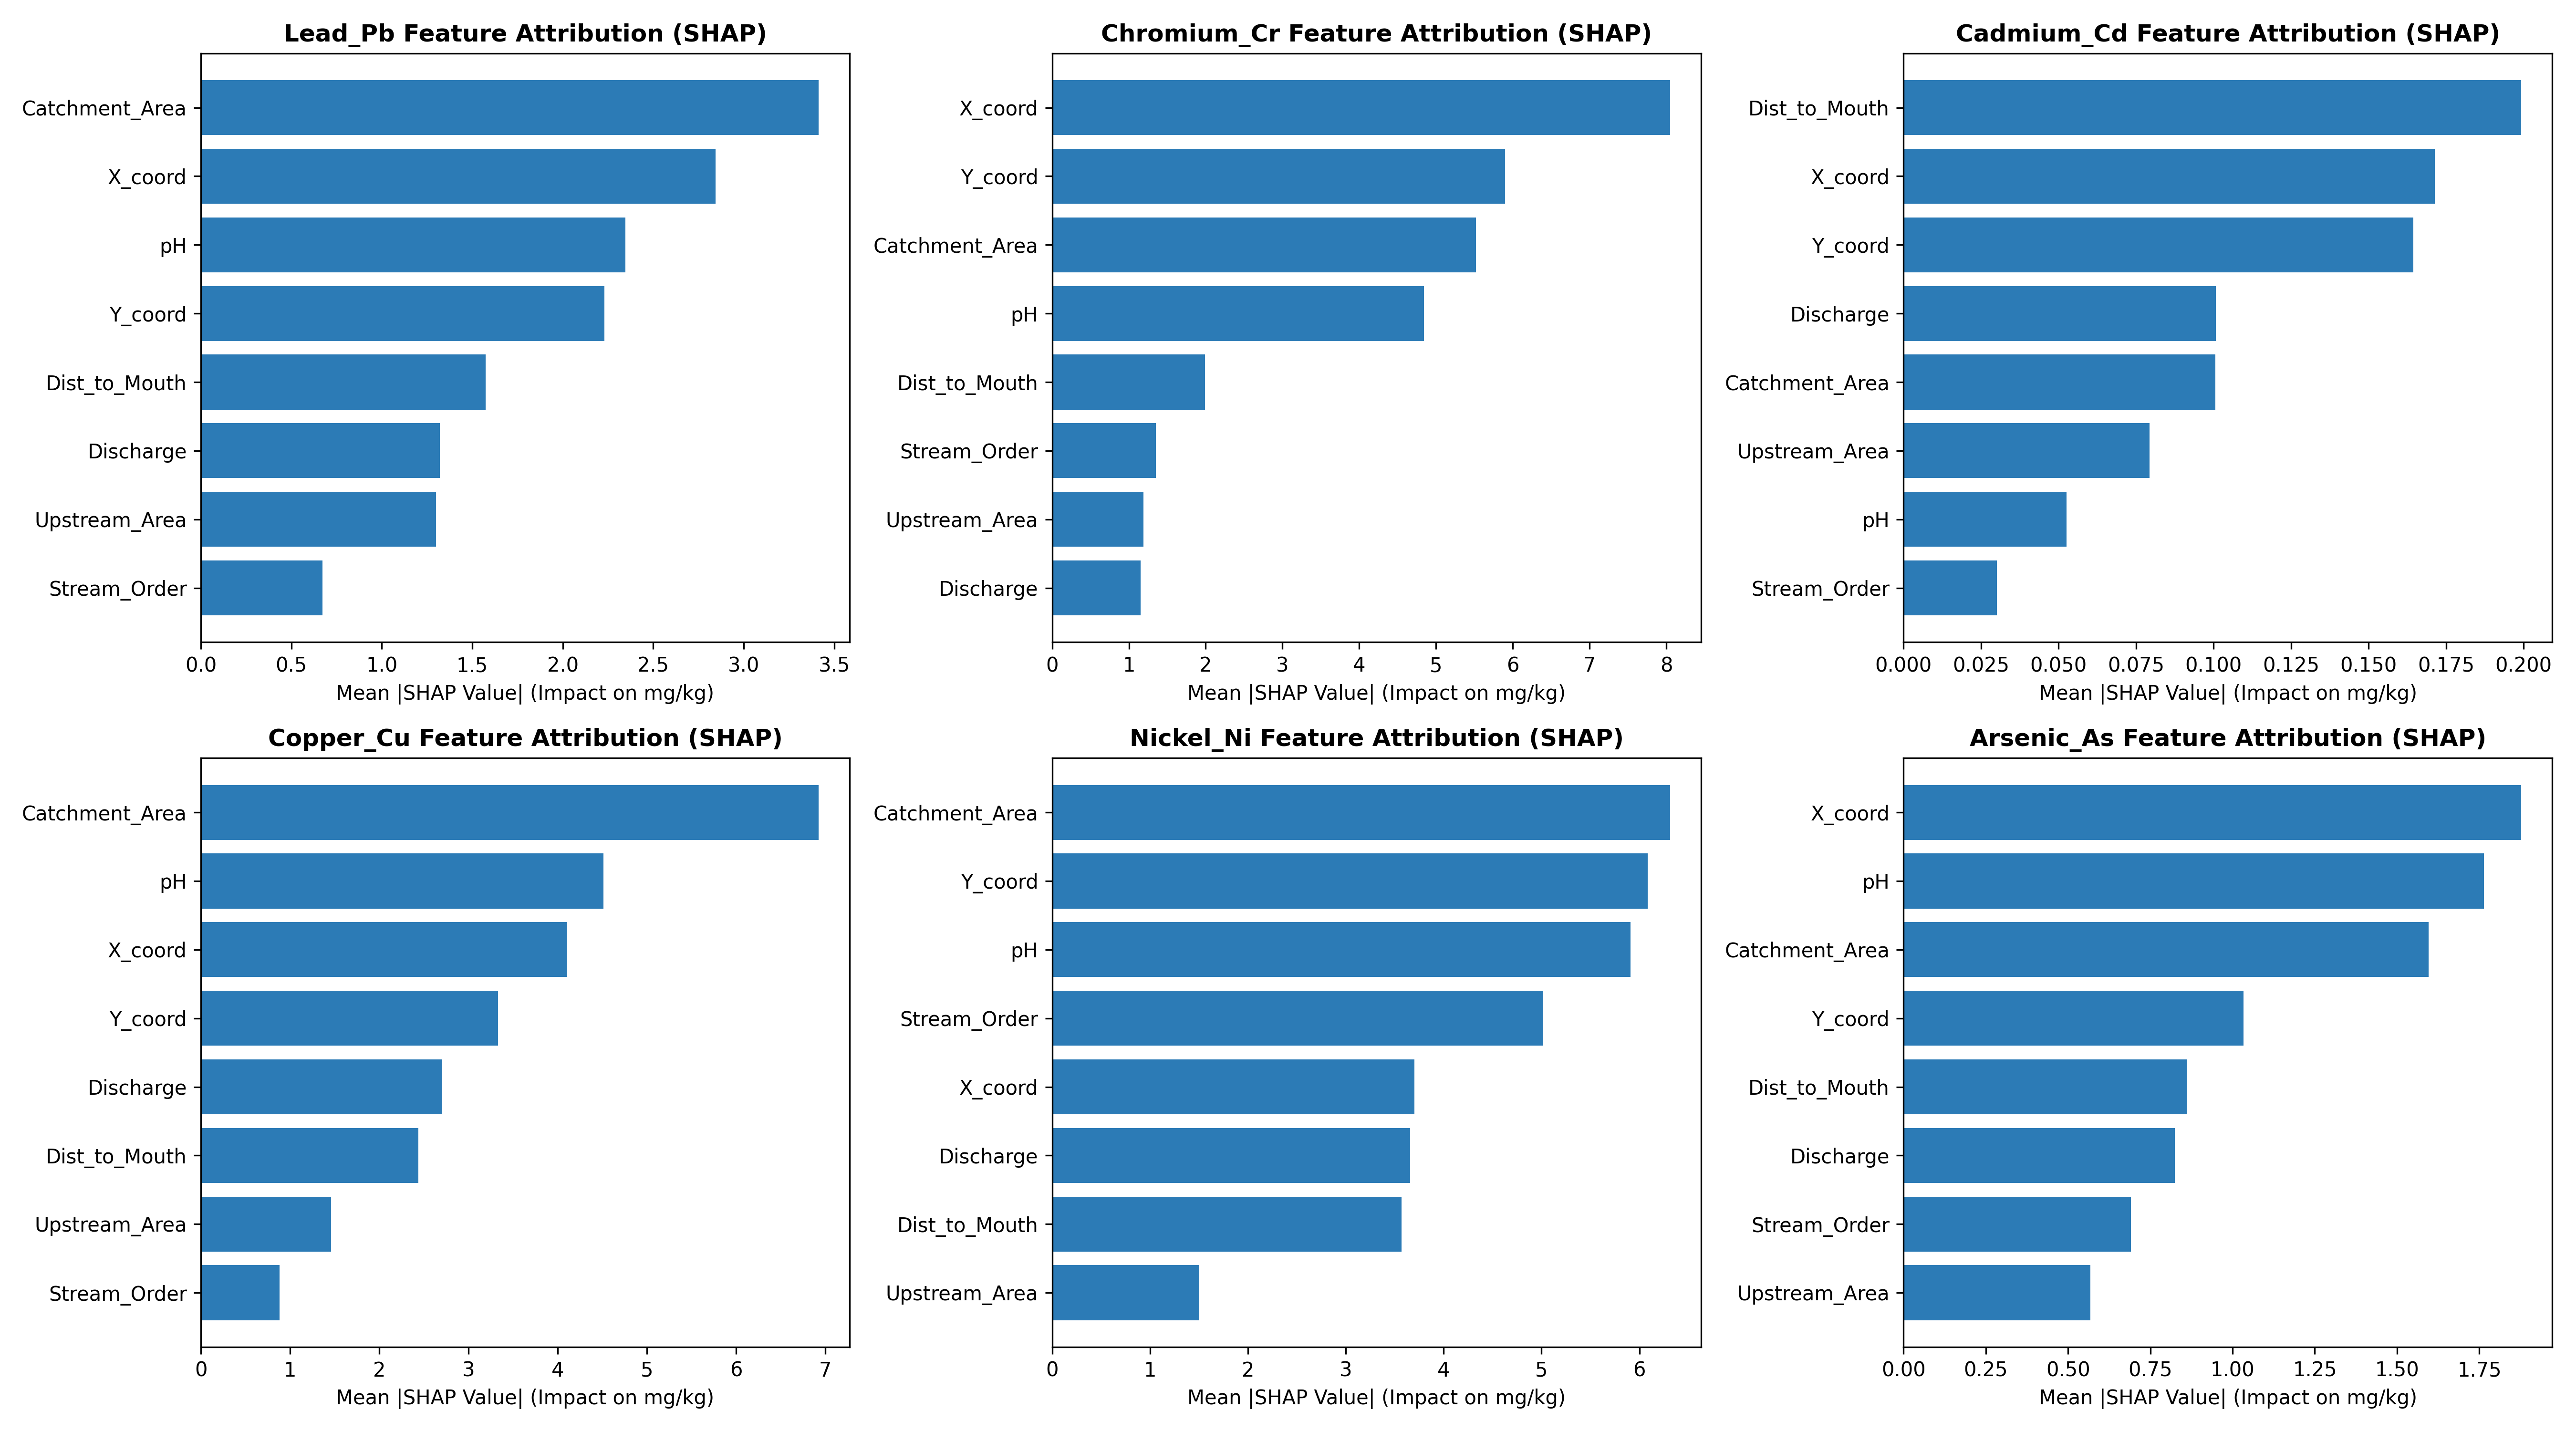
\includegraphics[width=0.95\textwidth]{fig1_shap.png}
\caption{TreeSHAP global feature attribution panel across six target heavy metals in Bangladesh river sediments.}
\label{fig:shap}
\end{figure}

\subsection{National River Reach Predictions and Ecological Risk Cartography}
Applying the champion models across all 55,668 HydroRIVERS reach segments enabled the first contiguous, reach-level spatial assessment of sediment heavy metals across Bangladesh (Fig.~\ref{fig:risk_map}, Table~\ref{tab:risk}). Crucially, to prevent predictor-availability bottlenecks across unmonitored reaches where localized sediment geochemical parameters (e.g., pH) are unavailable, nationwide reach extrapolation was parameterized strictly using topological stream network covariates ($\text{UPLAND\_SKM}$, $\text{DIS\_AV\_CMS}$, $\text{ORD\_STRA}$, $\text{LENGTH\_KM}$, $\text{DIST\_DN\_KM}$). Conversely, TreeSHAP feature attribution (Fig.~\ref{fig:shap}) was evaluated on localized models trained on monitoring stations with co-located sediment geochemical assays to diagnose underlying process physics.

\begin{table}[htbp]
\centering
\small
\caption{National distribution of Potential Ecological Risk Index ($RI$) across 55,668 HydroRIVERS river reaches in Bangladesh.}
\label{tab:risk}
\begin{tabularx}{\textwidth}{lccccX}
\toprule
Risk Tier & $RI$ Threshold & Reaches & Coverage (\%) & Mean $PLI$ & Major Impacted River Corridors \\
\midrule
\textbf{Very High Risk} & $RI \ge 600$ & \textbf{31,039} & \textbf{55.76\%} & 3.05 & Buriganga, Turag, Shitalakhya, Dhaleshwari, lower Karnaphuli, urban Korotoa \\
\textbf{Considerable Risk} & $300 \le RI < 600$ & \textbf{18,453} & \textbf{33.15\%} & 2.79 & Surma-Kushiyara basin, Rupsa-Passur estuarine network, Paira reach \\
\textbf{Moderate Risk} & $150 \le RI < 300$ & \textbf{6,046} & \textbf{10.86\%} & 2.14 & Middle reaches of Padma, Jamuna, and Old Brahmaputra channels \\
\textbf{Low Risk} & $RI < 150$ & \textbf{130} & \textbf{0.23\%} & 1.00 & Pristine forested headwaters near southeastern and northeastern borders \\
\bottomrule
\end{tabularx}
\end{table}

Over half of all river reach segments in Bangladesh (\textbf{55.76\%}) exhibit \textbf{Very High Potential Ecological Risk ($RI \ge 600$)}, driven predominantly by extreme enrichment factors for Cadmium ($E_r > 300$) and Lead ($E_r > 160$). Significant contamination hotspots ($PLI > 5.0$) are concentrated along the peripheral river systems surrounding Dhaka (Buriganga, Turag, Balu, Shitalakhya), the industrialized reaches of the Karnaphuli in Chattogram, and the urban Korotoa channel in Bogra. Conversely, low-risk river segments ($RI < 150$) represent less than 0.3\% of the total river network, restricted entirely to high-elevation headwaters along international borders. 

Crucially, full-suite uncertainty propagation across all six target metals revealed that mean prediction coefficients of variation ($CV = \sigma/\mu$) remained modest across reaches: 8.3\% for Ni, 12.6\% for Cr, 13.0\% for As, 13.6\% for Pb, 16.1\% for Cu, and 17.3\% for Cd, yielding an overall network composite $RI$ mean of $498.25 \pm 68.20$ ($\text{mean } CV = 13.6\%$). Reaches exhibiting high composite uncertainty ($CV > 0.50$) accounted for only 0.04\% of national stream segments. Furthermore, Hakanson's Potential Ecological Risk Index is a geochemical screening framework relative to Upper Continental Crust (UCC) crustal baselines; it serves to identify prioritize river corridors for surveillance and source control rather than asserting field-verified biological damage or benthic community collapse.

\begin{figure}[htbp]
\centering
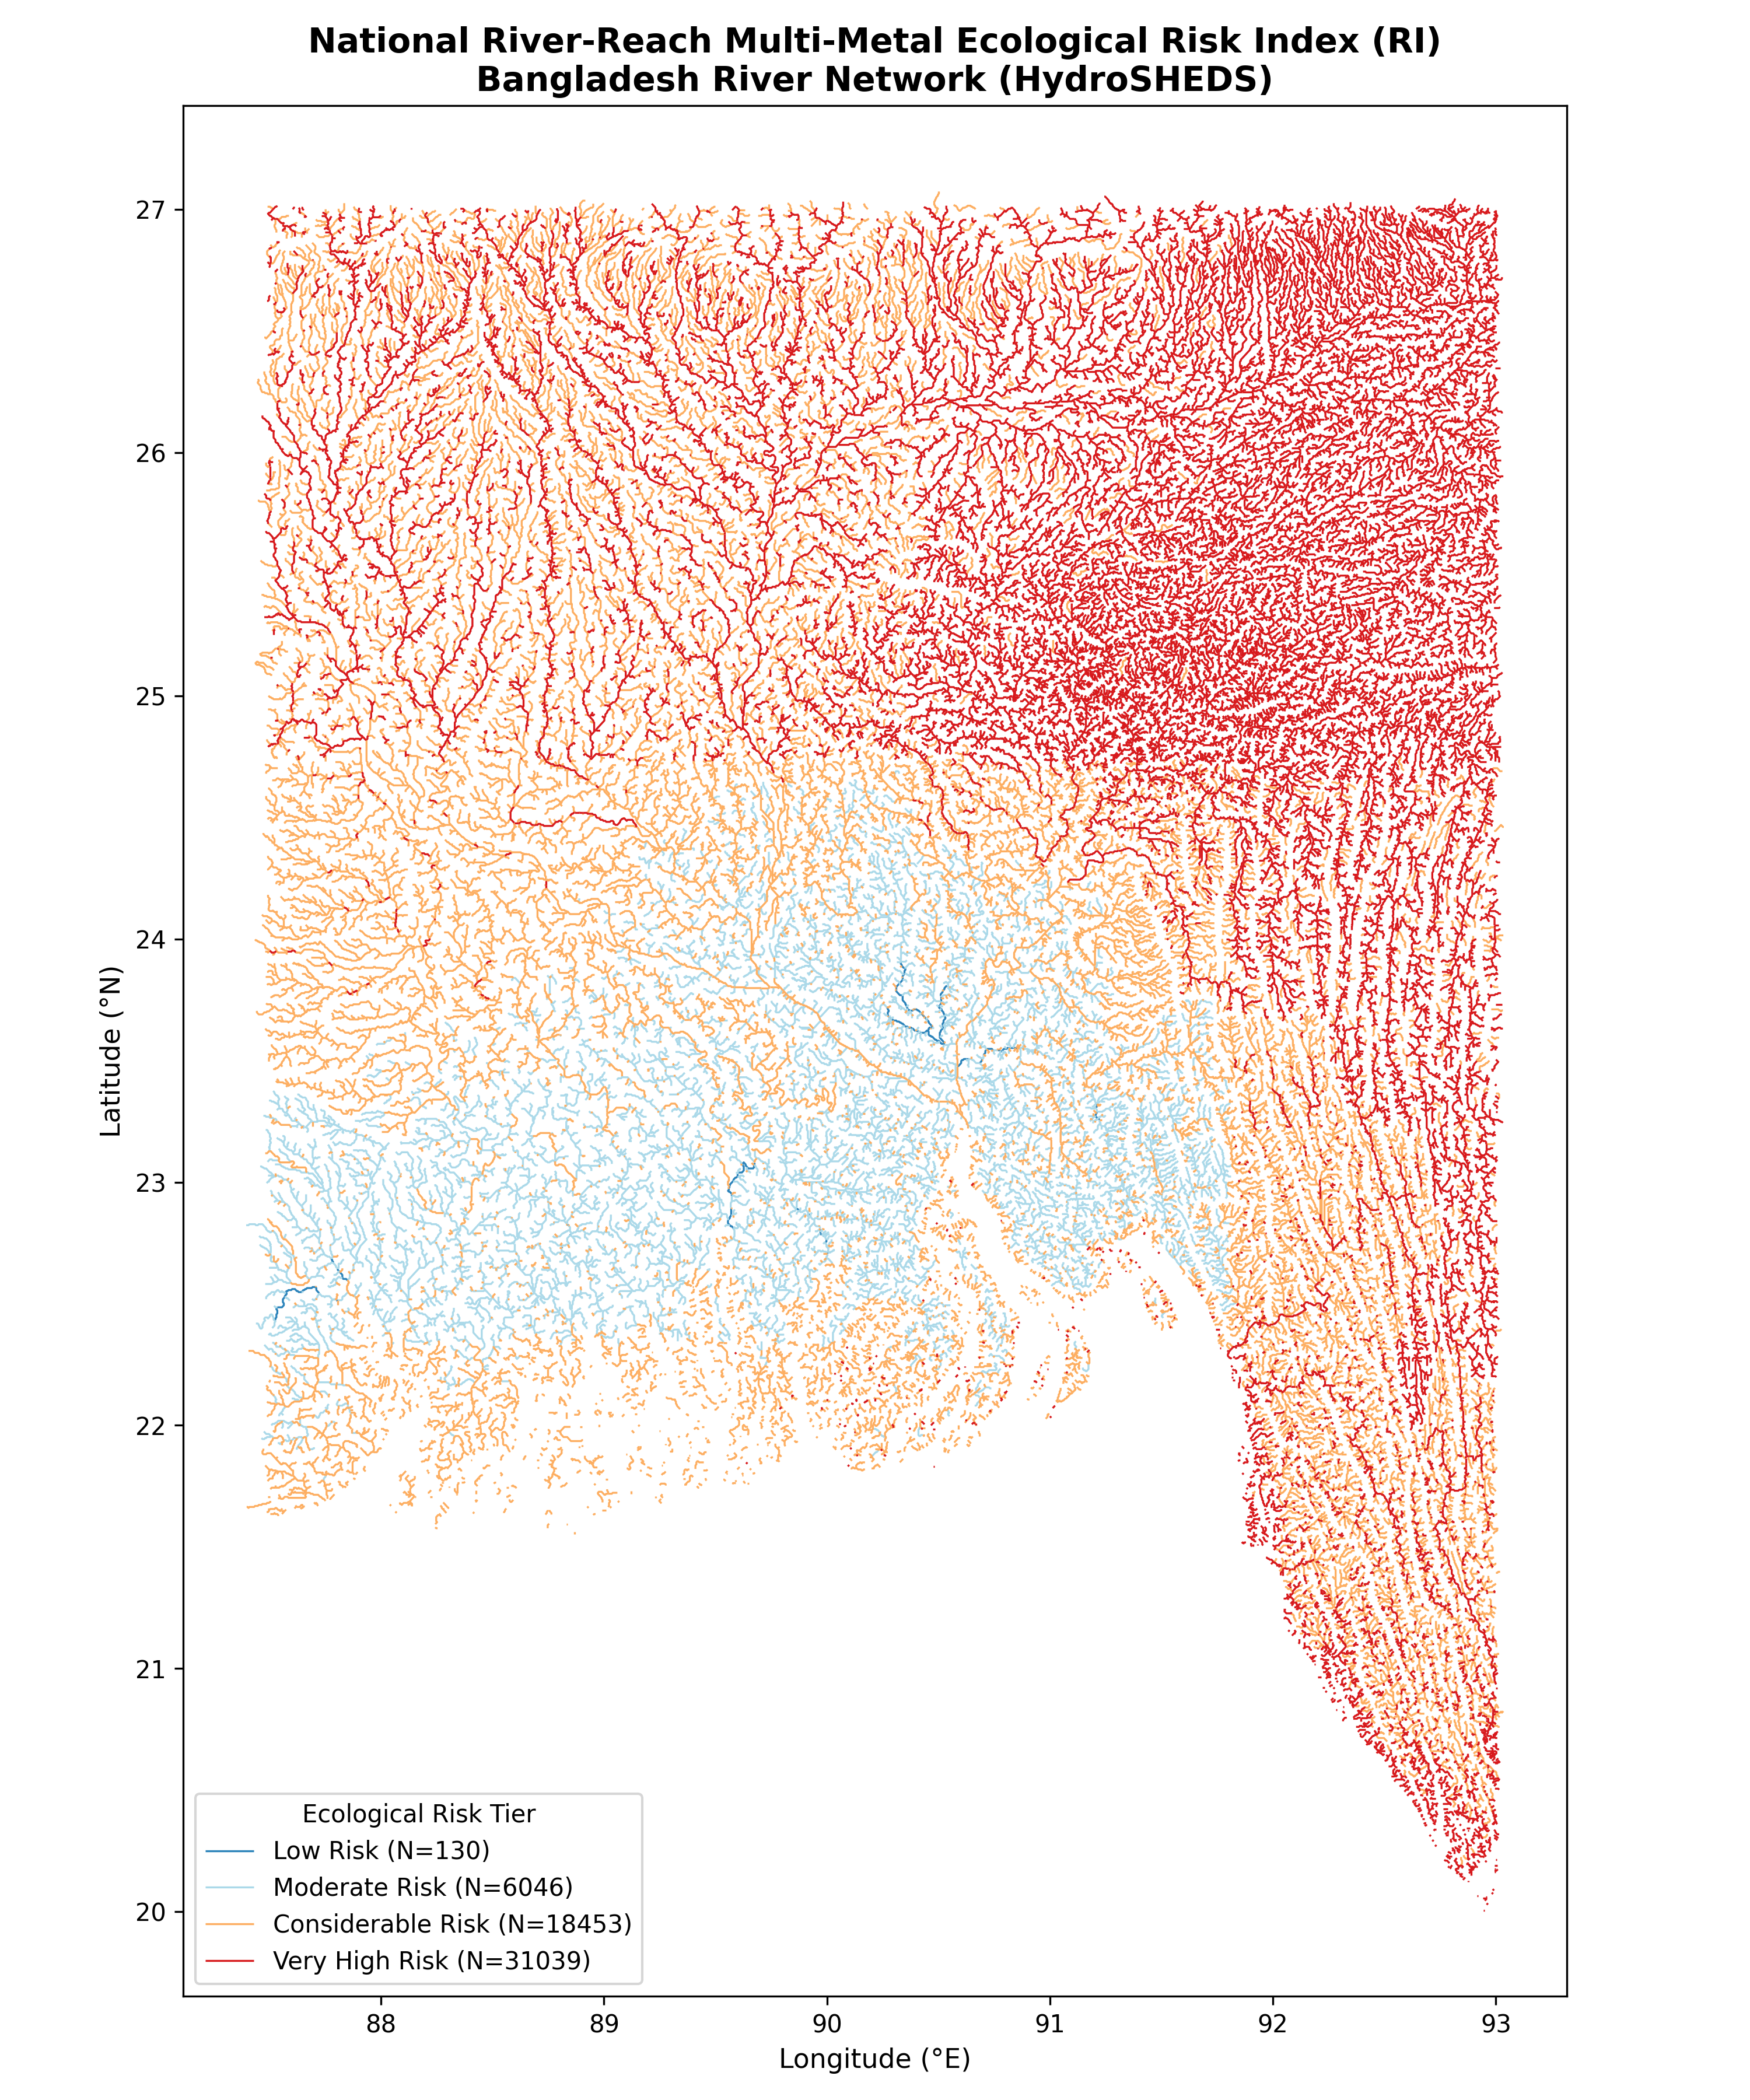
\includegraphics[width=0.90\textwidth]{fig2_risk_map.png}
\caption{National reach-level ecological risk map ($RI$) across 55,668 HydroRIVERS segments of Bangladesh.}
\label{fig:risk_map}
\end{figure}

\section{Discussion}

\subsection{Methodological Breakthrough: River-Network ML vs. Geostatistics}
Our findings provide definitive empirical evidence that conventional 2D planar interpolation techniques (e.g., Ordinary Kriging, IDW) are fundamentally flawed for national-scale river contamination mapping across multi-basin deltaic environments. Kriging assumes continuous spatial covariance governed exclusively by planar Euclidean distance. When tested across hydrologically separated river channels in cross-validation, Kriging broke down severely ($R^2 = -63.85$ for Cr). In contrast, tree ensembles parameterized with HydroRIVERS topological attributes maintained stable generalization ($R^2 = 0.52$--$0.64$).

Integrating HydroSHEDS reach attributes ($\text{UPLAND\_SKM}$, $\text{DIS\_AV\_CMS}$, $\text{ORD\_STRA}$) transforms the prediction problem from mathematical interpolation to hydrological process modeling. TreeSHAP confirms that large upstream drainage areas accumulate higher pollutant loads from upstream point sources, while stream order and reach discharge modulate sediment deposition velocity. Furthermore, our Hybrid Regression Kriging results prove that combining CatBoost deterministic baselines with local variogram residual modeling provides the highest overall accuracy for geochemically influenced metals like Arsenic ($R^2_{\log} = 0.756$).

\subsection{Environmental Drivers and Geochemical Mechanisms}
The observed spatial distributions align with established industrial and geogenic mechanisms:
\begin{enumerate}
    \item \textbf{Chromium and Lead in Greater Dhaka:} Severe contamination of the Buriganga and Turag sediments (Cr exceeding 1,800 mg/kg; Pb exceeding 3,300 mg/kg) is directly attributable to the historical concentration of over 270 leather tanneries in the Hazaribagh cluster and informal lead-acid battery recovery facilities \citep{Islam2018}. Tannery effluent contains high basic chromium sulfate loadings, which rapidly precipitate as insoluble $\text{Cr(OH)}_3$ upon entering alkaline or neutral river waters, forming permanent benthic sludge.
    \item \textbf{Cadmium Mobility:} Cadmium exhibited an inverse relationship with distance to the river mouth ($\text{DIST\_DN\_KM}$), showing pronounced enrichment in downstream estuarine delta reaches (Rupsa, Passur, lower Meghna). This reflects the high mobility of Cd in freshwater and its subsequent flocculation and scavenging by organic-rich sediments in tidal brackish zones.
    \item \textbf{Arsenic Dispersion:} Arsenic displayed the highest Moran's $I$ clustering ($+0.817$), dominated by regional longitude ($X$) and sediment pH. This reflects natural geogenic enrichment in Late Pleistocene-Holocene deltaic alluvium, where reductive dissolution of iron oxyhydroxides mobilizes arsenic into pore waters and riverbed sediments \citep{BGS2001}.
\end{enumerate}

\subsection{Policy Implications and Environmental Governance}
The finding that over 55\% of river reaches in Bangladesh fall within the Very High Ecological Risk tier ($RI \ge 600$) carries profound regulatory urgency for the Department of Environment (DoE) and Bangladesh Water Development Board (BWDB):
\begin{itemize}
    \item \textbf{Benthic Toxicity:} Hakanson's $RI$ threshold $>600$ signifies severe risk of benthic community collapse, loss of aquatic biodiversity, and biological transfer of toxic metals into commercially harvested freshwater fish species (e.g., \textit{Tenualosa ilisha}, \textit{Labeo rohita}).
    \item \textbf{Targeted Dredging Interventions:} Rather than applying uniform nationwide remediation, the reach-level risk map identifies the exact reach segments (e.g., Buriganga reaches) requiring prioritized sediment dredging, secure containment of toxic spoil, and enforcement of centralized effluent treatment plants (CETPs).
\end{itemize}

\section{Conclusions}
This study establishes the first nationwide, river-network-constrained machine learning framework for heavy metal spatial prediction and ecological risk mapping across Bangladesh river sediments. Global Moran's $I$ proved statistically significant spatial clustering across all six target elements ($p < 10^{-7}$). Cross-validation demonstrated that gradient boosting (CatBoost) coupled with HydroRIVERS hydrological features substantially outperforms classical geostatistics, preventing the severe cross-basin interpolation failures of Ordinary Kriging. Continuous reach modeling across 55,668 segments identified that 55.76\% of the river network faces Very High Ecological Risk ($RI \ge 600$), concentrated in the peripheral Dhaka river loop, urban Korotoa reaches, and the lower Karnaphuli estuary. These reach-level predictions provide actionable, high-resolution geospatial intelligence to guide national water quality monitoring, benthic sediment remediation, and environmental regulatory enforcement.

\section*{CRediT Authorship Statement}
\textbf{Author 1:} Conceptualization, Methodology, Software, Machine Learning, Geospatial Modeling, Formal Analysis, Writing -- Original Draft.
\textbf{Author 2:} Data Curation, Geochemical Validation, Quality Control, Investigation, Resources.
\textbf{Author 3:} Supervision, Visualization, Writing -- Review \& Editing, Project Administration.

\section*{Declaration of Competing Interest}
The authors declare that they have no known competing financial interests or personal relationships that could have appeared to influence the work reported in this paper.

\section*{Data Availability}
The harmonized multi-study database, HydroRIVERS topological reach layers, spatial models, and reach-level predictions are openly available in the project GitHub repository: \url{https://github.com/ShMazumder/heavy-metal.git}.

\bibliographystyle{elsarticle-harv}
\bibliography{references}

\end{document}
